\documentclass{standalone}
\usepackage{tikz}
\usepackage{ctex,siunitx}
\setCJKmainfont{Noto Serif CJK SC}
\usepackage{tkz-euclide}
\usepackage{amsmath}
\usetikzlibrary{patterns, calc}
\usetikzlibrary {decorations.pathmorphing, decorations.pathreplacing, decorations.shapes,}
\begin{document}
\small
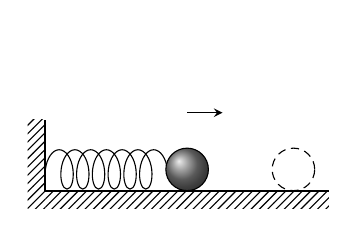
\begin{tikzpicture}[>=stealth,scale=0.9]
  \useasboundingbox(-0.25,-0.25)rectangle(4,2.3);
  \tikzstyle{spring}=[decorate,decoration={aspect=0.5, segment length=2mm, amplitude=2.5mm,coil}]
  \fill [pattern = north east lines] (-.25,-0.25) rectangle (0,1);
  \fill [pattern = north east lines] (0,-0.25) rectangle (4,0);
  \draw[thick](0,0)--(0,1);  
  \draw[thick](0,0)--(4,0); 
  \draw [spring](0,.3)--(1.8,.3);
  \filldraw [ball color=gray] (2,.3) circle  (0.3);
  \draw [densely dashed] (3.5,.3)circle  (0.3);
  \draw [->] (2, 1.1)--(2.5, 1.1);
\end{tikzpicture}
\end{document}